\section{Counts, baseline values and additional results}
\label{app:counts}

\paragraph{Counts} The KuaiRand-27K data contain 27,077 dataset users. In each split, 8,123 of them form the validation part and 18,954 the test
part. A test user is scored only if a candidate was clicked, which gives 15,809 to 15,913 scored test users per split. Pooled over the five splits,
22,612 distinct users are scored in at least one split. The headroom diagnostic of Section~\ref{sec:res-headroom} uses 22,661 users, all users with
a click in some candidate list. The difference of 49 users consists of users with a click who were in the validation part of all five splits, and
so are never scored.

\paragraph{Baseline values} Table~\ref{tab:methods} gives the mean and standard deviation of each method over the five splits, with the configurations
searched. The means are the means of the split means, as defined in Section~\ref{sec:protocol-stats}.

\begin{table}[tbp]
\centering
\footnotesize
\caption{Methods on KuaiRand-27K (temporal protocol, all users): mean and standard deviation of nDCG@10 over the five splits, and the configurations searched per split.}
\label{tab:methods}
\begin{adjustbox}{max width=\linewidth}
\begin{tabular}{lrrr}
\toprule
Method & Mean & SD & Configurations \\
\midrule
LEAF-LGN+DAX & 0.4854 & 0.0009 & 3,840 \\
LEAF-LGN & 0.4736 & 0.0002 & 12 \\
LEAF-LGN (separate search) & 0.4728 & 0.0011 & 197 \\
PW-LightGCN & 0.4634 & 0.0031 & 20 \\
PW-LightGCN+DAX & 0.4733 & 0.0012 & 3,200 \\
PW-LightGCN, re-trained on its selected configurations & 0.4652 & 0.0017 & 10 \\
r-AdjNorm & 0.4620 & 0.0008 & 8 \\
LightGCN & 0.4576 & 0.0031 & 4 \\
LightGCN+DAX & 0.4709 & 0.0010 & 960 \\
EASE & 0.4507 & 0.0009 & 27 \\
EASE+DAX & 0.4623 & 0.0010 & 8,640 \\
DIN & 0.4675 & 0.0007 & 4 \\
DIN+DAX & 0.4796 & 0.0015 & 1,280 \\
SIM & 0.4590 & 0.0009 & 4 \\
SIM+DAX & 0.4706 & 0.0018 & 1,280 \\
NAVIP & 0.4579 & 0.0020 & 4 \\
IPS-MF & 0.3765 & 0.0008 & 4 \\
DR-JL & 0.3823 & 0.0012 & 4 \\
MRDR & 0.3826 & 0.0008 & 4 \\
\bottomrule
\end{tabular}
\end{adjustbox}
\par\smallskip
\begin{minipage}{\linewidth}\raggedright\footnotesize Mean and SD are taken over the five split means. Configurations searched: backbone trainings times DAX configurations times values of $\gamma$. LEAF-LGN (separate search) is a search of the backbone alone, counted per training and epoch setting, so its count is not in the same unit. PW-LightGCN is, in each split, the best of its three variants on validation. \end{minipage}
\end{table}


\paragraph{KuaiRand-1K} Table~\ref{tab:1k} repeats the primary comparisons on KuaiRand-1K, with 842 test users pooled over the five splits. The
PW-LightGCN with DAX searches 6,400 configurations on this release, against 3,200 at 27K, which favours the baseline. The results are summarised in
Section~\ref{sec:res-1k}.

\begin{table}[tbp]
\centering
\footnotesize
\caption{KuaiRand-1K replication: LEAF-LGN+DAX against the PW-LightGCN with and without DAX (nDCG@10).}
\label{tab:1k}
\begin{adjustbox}{max width=\linewidth}
\begin{tabular}{lrrrcrr}
\toprule
Method or comparison & Mean & SD & Configs & Diff.\ [95\% hw] & NB $p$ & NB $p_{\mathrm{Holm}}$ \\
\midrule
LEAF-LGN+DAX & 0.4590 & 0.0038 & 3840 &  &  &  \\
PW-LightGCN & 0.4246 & 0.0043 & 20 &  &  &  \\
PW-LightGCN+DAX & 0.4358 & 0.0035 & 6400 &  &  &  \\
\midrule
LEAF-LGN+DAX minus PW-LightGCN &  &  &  & +37.58 [11.10] & 0.011 & $2.28\times10^{-2}$ \\
LEAF-LGN+DAX minus PW-LightGCN+DAX &  &  &  & +25.82 [9.66] & 0.007 & $2.18\times10^{-2}$ \\
PW-LightGCN+DAX minus PW-LightGCN &  &  &  & +11.76 [8.54] & 0.160 & $1.60\times10^{-1}$ \\
\bottomrule
\end{tabular}
\end{adjustbox}
\par\smallskip
\begin{minipage}{\linewidth}\raggedright\footnotesize Mean: the mean of the five split means. Diff.: the mean over the pooled test users of each user's paired difference (a user's difference is averaged over the splits in which the user is scored). The two are computed over different weightings, so a difference need not equal the difference of the two means shown. For example, the two means shown for LEAF-LGN+DAX and the PW-LightGCN differ by +34.3, against the paired difference of +37.58. KuaiRand-1K: 842 test users pooled over five splits (each split 30\% validation, 70\% test). The users are a subset of the 27K users, so this is a lower-power replication. The PW-LightGCN with DAX searches all 20 PW-LightGCN configurations on this release (6,400 configurations in total), whereas at 27K it searches the 10 selected ones (3,200); this favours the baseline. NB $p_{\mathrm{Holm}}$ is the Holm adjustment over the three comparisons of this table. Split differences ($\times10^{-3}$): LEAF-LGN+DAX minus PW-LightGCN: +36.7 +25.7 +35.6 +37.2 +36.6; LEAF-LGN+DAX minus PW-LightGCN+DAX: +21.3 +20.3 +23.7 +23.1 +27.8; PW-LightGCN+DAX minus PW-LightGCN: +15.4 +5.4 +11.9 +14.1 +8.8.\end{minipage}
\end{table}


\paragraph{Ablation gains} Figure~\ref{fig:ablate} shows the gains of Table~\ref{tab:ablate} with their 95\% half-widths and the five split values.

\begin{figure}[tbp]
\centering
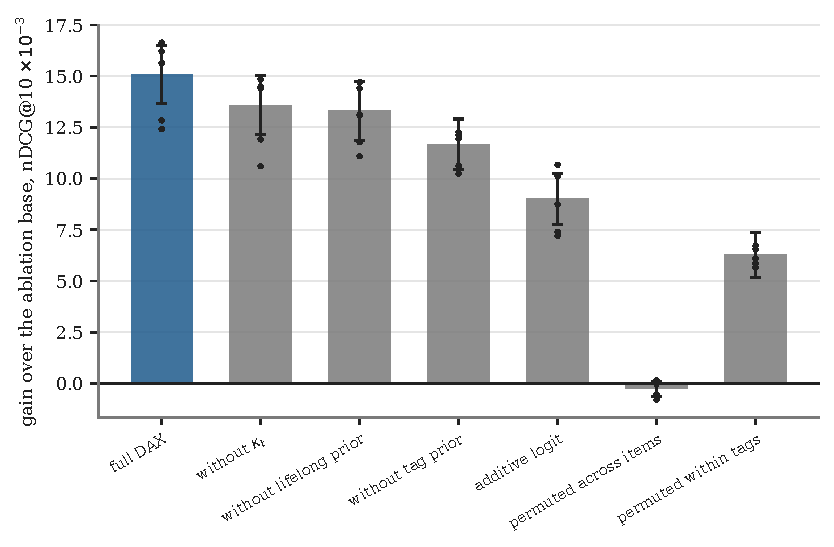
\includegraphics[width=0.8\linewidth]{figs/fig_ablate.pdf}
\caption{DAX ablations on KuaiRand-27K: gain over the LEAF-LGN base of the ablation search, with the 95\% half-width. Dots are the five splits. The
base is as in Table~\ref{tab:ablate}.}
\label{fig:ablate}
\end{figure}

\paragraph{Closest works} Table~\ref{tab:positioning} collects the works closest to the present one and states the difference from each.

\begin{table}[tbp]
\caption{Closest works and the difference from the present work.}
\label{tab:positioning}
\centering
\footnotesize
\raggedright
\begin{tabular}{p{3.4cm}p{4.2cm}p{5.4cm}}
\toprule
Work & What it estimates, and from which data & Difference from this work \\
\midrule
SIM \citep{pi2020sim}; TWIN \citep{chang2023twin} & CTR from lifelong sequences; policy logs; history and target share item ids & Exposure-conditional statistics; transfer to a disjoint pool through content keys; randomised test; SIM-hard is a baseline, TWIN is not \\
DIN \citep{zhou2018din} & Attention over the last 200 lifelong events; policy logs & Same comparison with DAX added; DIN is a baseline \\
Examination models \citep{richardson2007predicting,craswell2008cascade,chuklin2015clickmodels} & Click as examination times attractiveness; position or list scan & User and scenario examination; no position term; uniform-insertion target \\
Dynamic Bayesian network \citep{chapelle2009dbn} & Perceived versus actual relevance with satisfaction & No satisfaction state \\
Regression-EM \citep{wang2018regressionem,wang2016selection} & Position bias and relevance without randomisation; personal search & Item appeal under a uniform audience; generative fit by EM over user and scenario \\
ExpoMF \citep{liang2016exposure} & Latent exposure fitted by EM & Impressions are observed; latent examination given an impression \\
Unbiased learning to rank \citep{joachims2017unbiased} & Inverse-propensity weighted losses & Generative model instead of a weighted loss \\
Occupancy \citep{mackenzie2002occupancy} & Presence and detection from repeated surveys & Same likelihood structure; no recommender use found \\
Small-area estimation \citep{fay1979smallarea} & Small-area estimates & Used for one centre option of the DAX module \\
NAVIP \citep{kim2022navip} & Propensity-weighted propagation in LightGCN & No lifelong data; no examination model \\
KuaiRand evaluations \citep{gao2022kuairand,zhang2026categorymeans} & Random insertion as the test set & No out-of-pool lifelong history in the test \\
\bottomrule
\end{tabular}
\end{table}
